\documentclass[../template]{subfiles}

\begin{document}
\section{Flusso a costo minimo}
\begin{center}
    \begin{tikzpicture}[rotate=90, EdgeStyle/.style={->}]
        \Vertices[unit = 2]{circle} {1, 2, 3, 4, 5}
        \Edge[label=$5/9$](1)(2)
        \Edge[label=$15/4$](1)(4)
        \Edge[label=$2/3$](1)(3)
        \Edge[label=$3/11$](2)(4)
        \Edge[label=$2/4$](3)(4)
        ;
    \end{tikzpicture}
\end{center}
\subsection{Classificazione dei nodi}
Nei problemi di flusso a costo minimo, i nodi sono divisi in tre categorie, in base a $b_i$:
\begin{enumerate}
    \item Nodi sorgente: $b_i > 0$, in essi viene realizzato il prodotto.
    \item Nodi di transito: $b_i = 0$, il prodotto transita, senza variazioni
    \item Nodi destinazione: $b_i < 0$, dove il prodotto viene consumato.
\end{enumerate}
La proprietà $\sum_i^n b_i = 0$, quando non risulta valida, è forzabile aggiungendo un fittizio
con $b_{n+1} = -\sum_i^n b_i$, collegato a tutti i nodi sorgente, attraverso archi di costo 0 e capacità $+\infty$.

\subsubsection{Nel caso di archi con capacità illimitata}
\begin{wrapfigure}{R}{0pt}
    \centering
    \begin{tikzpicture}[rotate=90, EdgeStyle/.style={->}]
        \Vertices[unit=1.5]{circle}{1, 2, 3, 4, 5}
        \Edge[label=$5$, color=gray](1)(2)
        \Edge[label=$-2$, color=gray](1)(3)
        \Edge[label=$2$, color=red](1)(5)
        \Edge[label=$-4$, color=red](2)(3)
        \Edge[label=$0$, color=red](3)(4)
        \Edge[label=$6$, color=gray](4)(2)
        \Edge[label=$3$, color=red](4)(5)
        \Edge[label=$4$, color=gray](5)(3)
        ;
        \node[draw] at ([shift={(0:.7cm)}]1)   {$b=2$};
        \node[draw] at ([shift={(0:.7cm)}]2)   {$b=5$};
        \node[draw] at ([shift={(180:.7cm)}]3) {$b=1$};
        \node[draw] at ([shift={(180:.7cm)}]4) {$b=-4$};
        \node[draw] at ([shift={(0:.7cm)}]5)   {$b=-4$};
    \end{tikzpicture}
    \caption{$b_i$ sono indicati vicino al nodo}
    \label{graph:infty_flux}
\end{wrapfigure}
In un problema di flusso su rete a costo minimo una \textbf{base} coincide con un albero di supporto.
Ad ogni base è associabile una soluzione di base, ottenuta ponendo a 0 il flusso (quantità di
prodotto inviata) su tutti gli archi che non fanno parte della base.

\vspace{10pt}
Nell'esempio in figura \ref{graph:infty_flux} prendiamo come esempio la base $B_0 = \{\}$.
Prendiamo come esempio nella rete $G = (V, A)$ in figura \ref{graph:infty_flux}, la
base $B_0 = \{(1, 5), (2, 3), (3, 4), (4, 5)\}$ se poniamo nullo il flusso degli archi
non appartenenti alla base.
Di conseguenza, otteniamo che i flussi relativi agli archi sono:

\vspace{10pt}
\begin{tabular}{cc}
    (1, 5) = &2\\
    (2, 3) = &5\\
    (3, 4) = &6\\
    (4, 5) = &2
\end{tabular}
\\[10pt]
Se i flussi agli archi in base hanno valore non negativo,
\\
allora la soluzione è ammissibile, inoltre se i flussi sono tutti strettamente
maggiore di 0, allora si parla di soluzione non degenere.
Il costo totale di trasporto si calcola semplicemente sommando per ogni arco il prodotto tra
quantità di flusso e costo di trasporto. Nel caso di esempio:
\[
    c_{15} x_{15} + c_{23} x_{23} + c_{34} x_{34} + c_{45} x_{45} =
    2 \cdot 2 - 4 \cdot 5 + 0 \cdot 6 + 3 \cdot 2 = 10
\]
NOTA: questa è solo una possibile soluzione, per sapere se è ottimale occorre confrontarla con
le altre possibili soluzioni al problema.
\subsubsection{Coefficienti di costo ridotto}
I coefficienti a costo ridotto sono valori numerici associati agli archi che non fanno parte della
base, misurano la variazione del costo di trasporto al crescere dell'unità del valore del flusso
associato tale arco.
\end{document}
